\documentclass{beamer}
\usepackage{amsfonts,amsmath}
\usetheme{-statale}
\usefonttheme[onlymath]{serif}

\usepackage[italian]{babel}
\usepackage{bussproofs}
\usepackage{tabularx}
\usepackage{multirow}
\usepackage{tabularray}

\usepackage{float}
\usepackage{subcaption}
\usepackage{tikz}
\usetikzlibrary{positioning}
\usepackage{stmaryrd}
\usepackage{subcaption}
\usepackage{caption}
\usepackage{siunitx}

\EnableBpAbbreviations

\newcommand{\testcolor}[1]{\colorbox{#1}{\textcolor{#1}{test}}~\texttt{#1}}
\newcommand{\hrefcol}[2]{\textcolor{cyan}{\href{#1}{#2}}}

\definecolor{lightbluestatale}{RGB}{34, 167, 229}
\definecolor{darkbluestatale}{RGB}{0, 51, 102}

\newcommand{\llpar}{\rotatebox[origin=c]{180}{$\&$}}
\newcommand{\llten}{\otimes}
\newcommand{\llwith}{\&}
\newcommand{\llplus}{\oplus}
\newcommand{\llbot}{\bot}
\newcommand{\lltop}{\top}
\newcommand{\llone}{1}
\newcommand{\llzero}{0}

\titlebackground*{images/theme/background}

% ==================///==================///==================///
% ==================/// SPLASH PAGE
% ==================///==================///==================///

\title{Proof Search in Propositional Linear Logic via Boolean Constraints Satisfaction}
\course{Laurea Triennale in Informatica}
\author{Martino D'Adda}
\IDnumber{964827}

% ==================///==================///==================///
% ==================/// START PRESENTATION
% ==================///==================///==================///

\begin{document}

\maketitle

\footlinecolor{maincolor}

\section{Introduzione}
\begin{frame}{Calcolo dei sequenti}
	Il calcolo dei sequenti (G. Ghentzen, 1934) è un formalismo per rappresentare un calcolo logico e strutturarne dimostrazioni.
	I concetti principali sono due:
	\begin{itemize}
		\item \onslide<2->{il sequente $\Delta \vdash \Gamma$, che rappresenta una implicazione tra la congiunzione e la disgiunzione di sequenze di formule;}
		\item \onslide<3->{la regola, che descrive come si possono manipolare i sequenti, ad esempio
			$$
			\AXC{$\overbrace{\Delta \vdash \phi', \Gamma}^{\Pi'}$}
			\AXC{$\overbrace{\Delta \vdash \phi'', \Gamma}^{\Pi''}$}
			\LeftLabel{$\wedge$}
			\BIC{$\underbrace{\Delta \vdash \phi' \wedge \phi'', \Gamma}_{\Pi}$}
			\DP
			$$
		stabilisce che se valgono $\Pi'$ e $\Pi''$, allora vale $\Pi$.}
	\end{itemize}
\end{frame}

\begin{frame}{Calcolo dei sequenti cont'd}
	Una dimostrazione consiste in un albero avente come radice il sequente da dimostrare e ottenuto concatendo regole.
	$$
	\AXC{}
	\LeftLabel{$A$}
	\UIC{$a, b \vdash b$}
	\AXC{}
	\LeftLabel{$A$}
	\UIC{$a, b \vdash a$}
	\LeftLabel{$\wedge_R$}
	\BIC{$a, b \vdash b \wedge a$}
	\LeftLabel{$\wedge_L$}
	\UIC{$a \wedge b \vdash b \wedge a$}
	\DP
	$$
	Un \textbf{theorem prover} è un programma che, dato un sequente, prova a costruirne la dimosrazione.
	Nello specifico un theorem prover è detto bottom-up se parte dal sequente da dimostrare, e lo continua a scomporre applicando le regole ``al contrario''.
\end{frame}

\begin{frame}{Logica lineare}
	La \textbf{logica lineare} (J.-Y. Girard, 1987) è una logica la cui caratteristica principale è che è generalmente proibita la duplicazione o l'eliminazione di formule, operazioni che altrimenti sono spesso lasciate implicite.
	Questa scelta porta ad alcune proprietà particolari, tra cui la duplicazione dei connettivi della logica classica secondo due interpretazioni diverse, una detta moltiplicativa e l'altra additiva.
	\begin{center}
		\begin{tabular}{c|cccc|}
			\cline{2-5}
				 & $\wedge$ & $\vee$   & $\top$   & $\bot$ \\
			\cline{2-5}
			\noalign{\vskip\doublerulesep
         			\vskip-\arrayrulewidth}
			\cline{2-5}
			Molt.    & $\llten$  & $\llpar$  & $\llone$ & $\llbot$ \\
			Add.	 & $\llwith$ & $\llplus$ & $\lltop$ & $\llzero$ \\
			\cline{2-5}
		\end{tabular}
	\end{center}
\end{frame}
\begin{frame}{Splitting}
	Durante il proof searching bottom-up uno dei problemi pincipali è quello dello \textbf{splitting}.
	$$
	\AXC{$\vdash \Delta', \phi'$}
	\AXC{$\vdash \Delta'', \phi''$}
	\LeftLabel{$\llten$}
	\BIC{$\vdash \Delta', \Delta'', \phi' \llten \phi''$}
	\DP
	$$
	La scomposizione dei moltiplicativi, ad esempio nella regola del tensore di cui sopra, comporta il partizionamento di $\Delta$ in $\Delta'$ e $\Delta''$ per continuare la dimostrazione.
	Questa operazione può richiedere un numero esponenziale di tentativi.

	Nel 2001 D.Pym e J.Harland propongono un metodo per gestire lo splitting utilizzando vincoli booleani generati a partire da espressioni associate a ogni singola formula.
\end{frame}

\section{Il calcolo}
% ==================///==================///==================///
% ==================/// BODY'S PRESENTATION
% ==================///==================///==================///

% \input{sections/introduction}

% \input{sections/analysis}

% \input{sections/conclusions}

\begin{frame}{Focusing e normalizzazione}
	Partendo dal calcolo citato sopra di D.Pym e J.Harland, abbiamo applicato due classiche modifiche nell'ambito del proof searching (i.e. normalizzazione e focusing).
	Di questo nuovo calcolo -- che chiameremo $C$ -- abbiamo poi mostrato la correttezza esibendo una traduzione verso un calcolo intermedio ($A$) tale che il seguente diagramma commuta:
	\begin{center}
		\begin{tikzpicture}
			\node (our-calc) {$C$};
			\node (andreoli) [right=of our-calc] {$A$};
			\node (classic)  [below=of andreoli] {$LL$};

			\draw[->] (our-calc) to node[above] {\tiny $\llbracket - \rrbracket_C$} (andreoli);
			\draw[->] (andreoli) to node[right] {\tiny $\llbracket - \rrbracket_A$} (classic);
			\draw[->, dashed] (our-calc) to node[below left] {\tiny $\llbracket - \rrbracket_A \circ \llbracket - \rrbracket_C$} (classic);
		\end{tikzpicture}
	\end{center}
	con $LL$ il calcolo classico della logica lineare e $\llbracket - \rrbracket$ le rispettive traduzioni.
\end{frame}
\begin{frame}{Implementazione}
	Per il calcolo di sopra sono state scritte:
	\begin{itemize}
		\item<2-> un'implementazione in SWI-Prolog;
		\item<3-> un generatore di test in OCaml;
		\item<4-> una libreria per il testing e il benchmarking in Python.
	\end{itemize}
	\onslide<5->{Infine l'infrastruttura per tutti i programmi di sopra è stata gestita con Nix.}
	\begin{center}
		\begin{tabular}{*{4}{wc{2cm}}}
			\onslide<2->{
\includegraphics[width=1.5cm]{images/prolog-logo}} &
			\onslide<3->{
\includegraphics[width=1.5cm]{images/ocaml-logo}} &
			\onslide<4->{
\includegraphics[width=1.5cm]{images/python-logo}} &
			\onslide<5->{
\includegraphics[width=1.5cm]{images/nix-logo}} \\
		\end{tabular}
	\end{center}
\end{frame}

\section{Conclusione}
\begin{frame}{Risultati -- caso moltiplicativo}
	\begin{columns}
		\begin{column}{.5\textwidth}
	Una volta implementato il prover lo si è confrontato con altri due prover basati a grandi linee sullo stesso algoritmo (i.e. bottom-up focused proof search): llprover (1997) e APLL (2016).
	Nel caso moltiplicativo -- quello principalmente soggetto al problema dello splitting -- i risultati sono buoni:
		\end{column}
		\begin{column}{.5\textwidth}
			\begin{figure}[H]
				\centering
				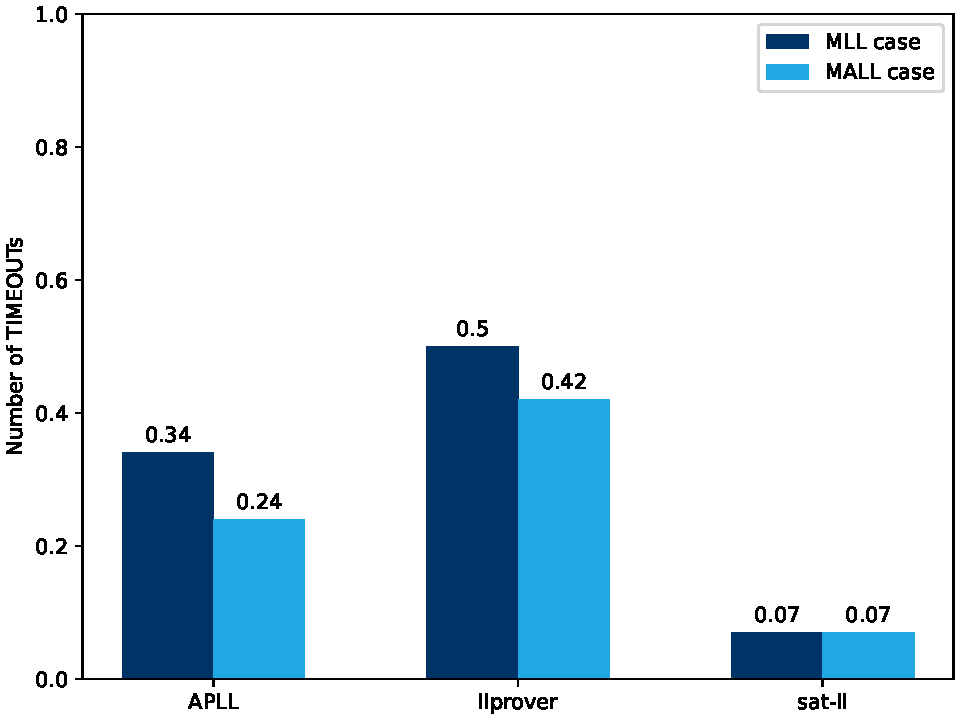
\includegraphics[scale=.4]{images/graph}
			\end{figure}
		\end{column}
	\end{columns}
\end{frame}
\begin{frame}{Risultati -- caso generale}
	Nel caso dei test esponenziali utilizziamo due dataset preesistenti e vediamo che i risultati si livellano:
	\begin{table}[h!]
		\begin{subtable}{\textwidth}
			\centering
			{\footnotesize
			\begin{tabular}{ | l c c c c c c | }
				\hline
				\textbf{prover} & \textbf{timeouts} & \textbf{failures} & \textbf{successes} & \textbf{success rate} & \textbf{avg. (succ.)} & \textbf{avg. (tot.)} \\
				\hline
				\hline
				APLL     & $0$  & $17$ & $71$ & \color{darkbluestatale}{$\approx 0.80$} & \qty{0.035}{\second} & \qty{0.326}{\second} \\
				llprover & $20$ & $6$  & $62$ & \color{darkbluestatale}{$\approx 0.70$} & \qty{0.981}{\second} & \qty{2.179}{\second} \\
				sat-ll   & $5$  & $15$ & $68$ & \color{darkbluestatale}{$\approx 0.77$} & \qty{0.443}{\second} & \qty{0.496}{\second} \\
				\hline
			\end{tabular}
			}
			\caption{Output per KLE-cbv}
			\label{table:KLE-cbv}
		\end{subtable}
		\begin{subtable}{\textwidth}
			\centering
			{\footnotesize
			\begin{tabular}{ | l c c c c c c | }
				\hline
				\textbf{prover} & \textbf{timeouts} & \textbf{failures} & \textbf{successes} & \textbf{success rate} & \textbf{avg. (succ.)} & \textbf{avg. (tot.)} \\
				\hline
				\hline
				APLL     & $0$  & $16$ & $72$ & \color{darkbluestatale}{$\approx 0.80$} & \qty{0.037}{\second} & \qty{0.055}{\second} \\
				llprover & $20$ & $6$  & $62$ & \color{darkbluestatale}{$\approx 0.70$} & \qty{1.709}{\second} & \qty{3.253}{\second} \\
				sat-ll   & $4$  & $18$ & $66$ & \color{darkbluestatale}{$\approx 0.75$} & \qty{0.130}{\second} & \qty{0.185}{\second} \\
				\hline
			\end{tabular}
			}
			\caption{Output per KLE-cbn}
			\label{table:KLE-cbn}
		\end{subtable}
	\end{table}
\end{frame}

% ==================///==================///==================///
% ==================/// END PRESENTATION
% ==================///==================///==================///

\backmatter[notitle]

%=======================================================================

\end{document}
